\documentclass[draftcls,onecolumn]{IEEEtran}

%% INCLUDING THE PREAMBLE
%%%%%%%%%%%%%%%%%%%%%%%%%%%%%%%%%%%%%%%%%%%%%%%%%%%%%%%%%%%%%%%%%%%%%%%%%%%
%                                                                         %
%                                 PREAMBLE                                %
%                                                                         %
%%%%%%%%%%%%%%%%%%%%%%%%%%%%%%%%%%%%%%%%%%%%%%%%%%%%%%%%%%%%%%%%%%%%%%%%%%%

%% PACKAGES
\usepackage[]{lineno}
%\linenumbers
\usepackage[usenames,dvipsnames]{xcolor}
\usepackage{microtype}
\usepackage[obeyDraft]{todonotes}
\usepackage{fancyvrb}
\VerbatimFootnotes
\usepackage{algorithmic}

%% GRAPHICS RELATED
\usepackage{graphicx}
\usepackage[outdir=./tmp/]{epstopdf}
\graphicspath{{../images/}{./}{./tmp/}}
\DeclareGraphicsExtensions{.eps, .pdf, .jpeg, .png,}

%% CPATION SETUP
\usepackage{float}
\usepackage{caption}
\usepackage{subcaption}
\captionsetup{belowskip=12pt,aboveskip=4pt}


%% BIBLIOGRAPHY
\bibliographystyle{ieeetr}

%% UNITS
\usepackage{siunitx}

%% EQUATIONS
\usepackage{amsmath}
%\numberwithin{equation}{section}

%% HYPERLINKS
\usepackage[debug]{hyperref}

%%%%%%%%%%%%%%%%%%%%%%%%%%%%%%%%%%%%%%%%%%%%%%%%%%%%%%%%%%%%%%%%%%%%%%%%%%%
%                                                                         %
%                             Listing Setup                               %
%                                                                         %
%%%%%%%%%%%%%%%%%%%%%%%%%%%%%%%%%%%%%%%%%%%%%%%%%%%%%%%%%%%%%%%%%%%%%%%%%%%
\usepackage{listings}
\lstset{ %
    language=C++,
    basicstyle=\footnotesize\ttfamily,
    numbers=left,
    numberstyle=\tiny\color{gray},
    stepnumber=2,
    numbersep=5pt,
    backgroundcolor=\color{white},
    showspaces=false,
    showstringspaces=false,
    showtabs=false,
    frame=single,
    rulecolor=\color{black},
    tabsize=2,
    breaklines=true,
    breakatwhitespace=false,
    title=\lstname,
    keywordstyle=\color{blue},
    commentstyle=\color{OliveGreen},
    stringstyle=\color{orange}
}
\DeclareCaptionFont{white}{\color{white}}
\DeclareCaptionFormat{listing}{\colorbox[cmyk]{0.43, 0.35, 0.35, 0.01}{\parbox{\dimexpr\textwidth-2\fboxsep\relax}{#1#2#3}}}
\captionsetup[lstlisting]{format=listing,labelfont=white,textfont=white,singlelinecheck=false,margin=0pt,font={bf,footnotesize}}
%\lstnewenvironment{code}[1][]%
%{ \noindent\minipage{\linewidth}
%	\lstset{#1}
%}
%{\endminipage}
%% USER COMMANDS
\usepackage{isotope}
\newcommand{\iso}{\isotope}
\newcommand{\figurewidth}{\textwidth}
\newcommand{\micron}{$\mu$m}



%%%%%%%%%%%%%%%%%%%%%%%%%%%%%%%%%%%%%%%%%%%%%%%%%%%%%%%%%%%%%%%%%%%%%%%%%%%
%                                                                         %
%                                Start of Document                        %
%                                                                         %
%%%%%%%%%%%%%%%%%%%%%%%%%%%%%%%%%%%%%%%%%%%%%%%%%%%%%%%%%%%%%%%%%%%%%%%%%%%
\begin{document}
\title{Layered Detectors}
\author{Matthew J. Urffer}
\date{\today}
\maketitle


% Tables of Contents, Figures, Tables
\listoftodos
\tableofcontents
\listoffigures
\listoftables
\lstlistoflistings
%%%%%%%%%%%%%%%%%%%%%%%%%%%%%%%%%%%%%%%%%%%%%%%%%%%%%%%%%%%%%%%%%%%%%%%%%%%
%                                                                         %
%                              Start of Content                           %
%                                                                         %
%%%%%%%%%%%%%%%%%%%%%%%%%%%%%%%%%%%%%%%%%%%%%%%%%%%%%%%%%%%%%%%%%%%%%%%%%%%
\section{Introduction}

It was observed in repeating the neturon fraction above the gamma LLD that there was signficant disgrepancy between a film mounted on a thin PMMA disc and a film mounted on a thick UVT (ultra-violet tranpsarent) aryclic disc, as shown in \autoref{tab:PSFractionRepeatMeas}.
This was observed for two differnet films thickness (\SI{25}{\um} and \SI{50}{\um}) with each film being 10\% LiF in a polystyrene matrix.
\begin{table}
	\centering
	\caption[PS Film Neutron Fraction Measurments]{Neutron Response Measurments of Polystyrene Films.  Note that the \SI{150}{\um} Film has repeatable measurments, while the \SI{25}{\um} and \SI{50}{\um} do not.}
	\label{tab:PSFractionRepeatMeas}
\begin{tabular}{m{2cm} | m{1cm} m{1.5cm} m{1.5cm} m{2cm} m{2cm}}
Name&Thickness&Gamma LLD \num{1E-6} (channel) & Neutron Count Rate (cps) & Neutron Count Rate Above Gamma LLD & Neutron Fraction\\
\hline
\hline
\verb+PS_LiF(10.3)_PPO(4.90)-Annealed_25um_29MayFeb2012+ & 25 & 772&6.336&0.207&0.0327 \\
\verb+PS_LiF(9.66)_PPO(4.58)-Annealed_26um_19Jan2012+    & 26&1100&9.742&5.073&0.5207 \\
\hline
\verb+PS_LiF(9.95)_PPO(5.11)_50um_24Jan2012+             &50&1352&20.686&6.453&0.3120 \\
\verb+PS_LiF(10)_PPO(5)_50um_28Feb2013+		  &50&1365&12.489&0.245&0.0196 \\
\hline
\verb+PS_LiF(9.88)_PPO(5)_151um_20Aug2011+	          &151&2386&53.872&0.195&0.0036 \\
\verb+PS_LiF(10)_PPO(4.94)_151um_25July2011+	          &151&2385&60.615&0.189&0.0031 \\
\end{tabular}
\end{table}
It is observed from \autoref{tab:PSFractionRepeatMeas} that the gamma measurments as indicated by the MLLD are stable while the neutron count rate is not. 
It is shown in \autoref{fig:NeutronCountRateRepeat} that there is a distinict difference between the PMMA mounted and UVT mounted disc, with the PMMA mounted films having a much lower performance.

\begin{figure}
  \centering
  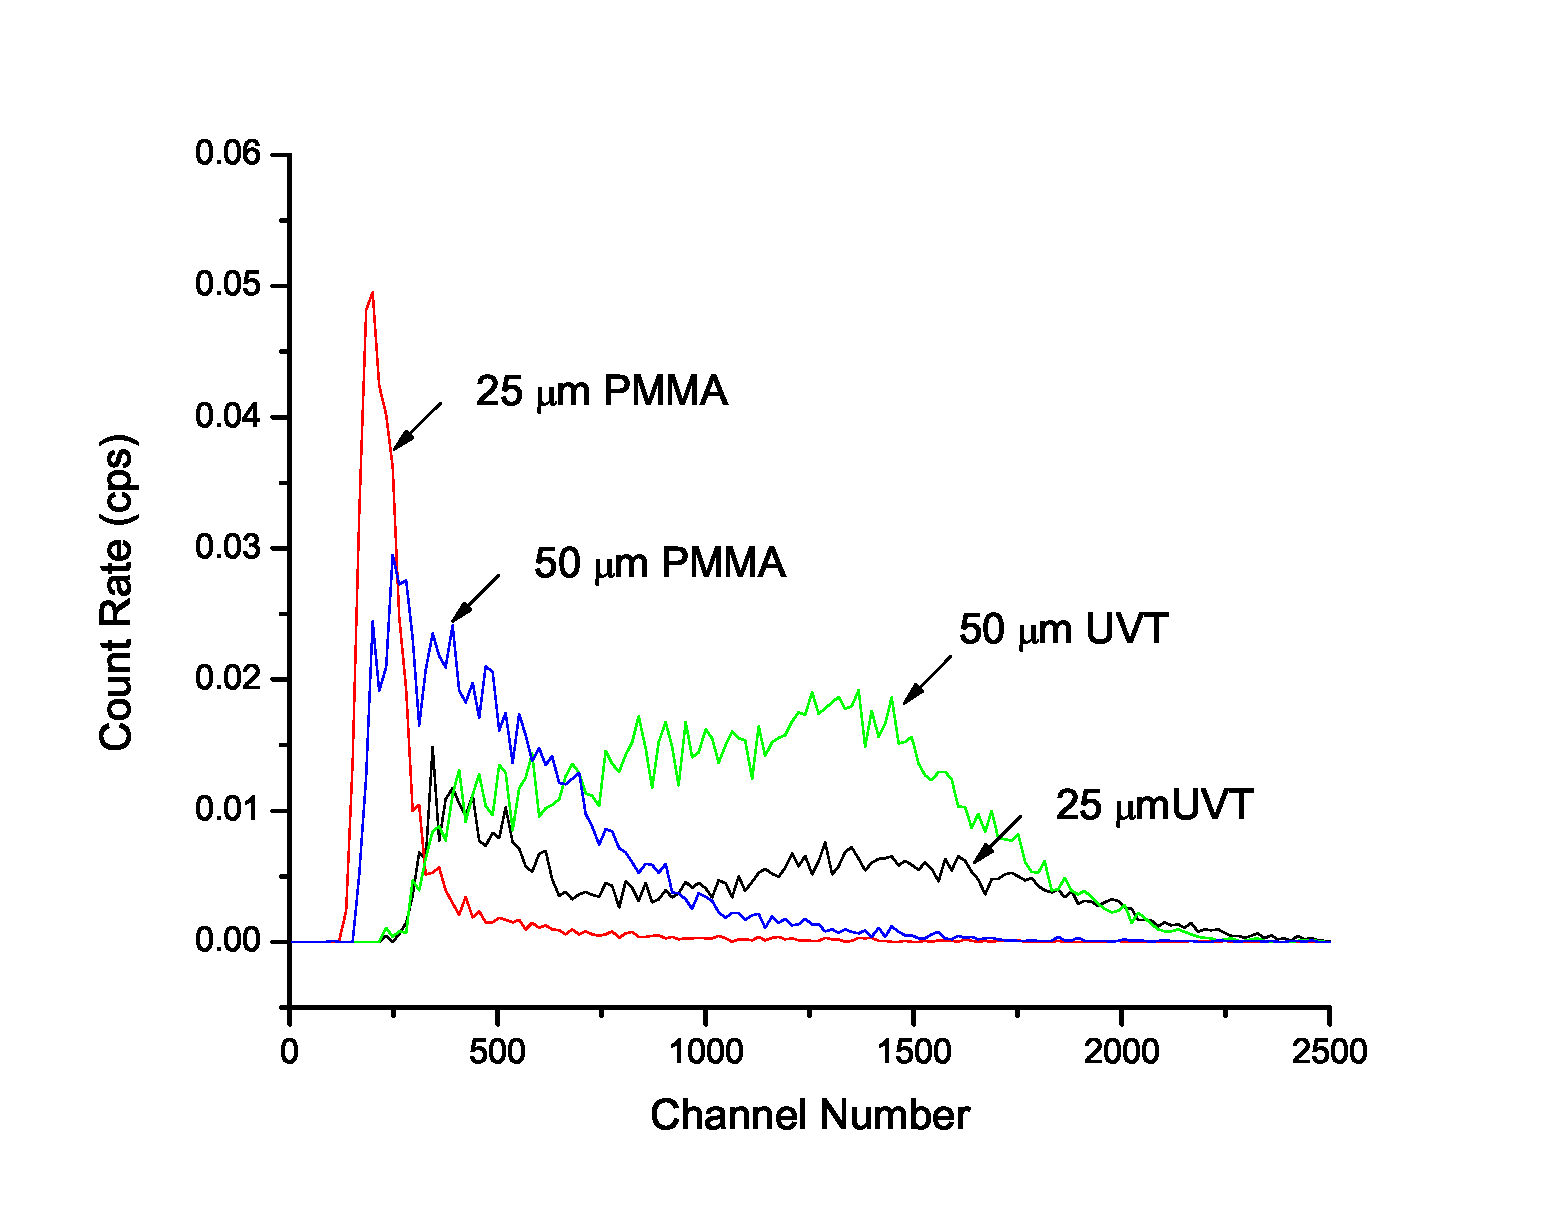
\includegraphics[width=\textwidth]{UVTPMMA_CountRate}
  \caption[Neutron Spectra of UVT mounted and PMMA mounted films]{Neutron spectra of UVT mounted and PMMA mounted films.  It is evident that both UVT mounted films have the same endpoint (differing mostly in count rate) while the PMMA films have a much lower neutron endpoint and a differnet spectra shape.}
  \label{fig:NeutronCountRateRepeat}
\end{figure}
Several differnet causes of this disgregency were considered:
\begin{itemize}
  \item energy deposition by charged particles not being fully absorbed in the thin disc,
  \item light propogation through the aryclic disc being attenuated,
  \item and adverse chemical reactions in the PMMA disc.
\end{itemize}

It was quickly ruled out that the energy deposition by the reaction products could not be repsonsible.
As both materials are made of the same constituents it is reasonable to expect that the reflection of electron from the disc back unto the film would be very similar.
\todo[inline]{I could verify this with a quick GEANT4 sim, changing the thickness of the backing}.
In addition, a \iso[36]{Cl} source was placed directly on the PMT and no counts above background were absorved, thus making it unlikely that electrons were escaping the film and interacting directly with the photo-diode on the PMT.

\section{Methods}
From the arguments made above it was determined that the cause of this disgrepency must be either light propagaation in the disc, differnet material compsotions, or addiation chemistry occuring between the cast film and disc upon which it was cast.
In order to determine if it was light propogation throught the films two sets of experiments were completed in which it was attempted to replicate a thin film as mounted on a thicker disc, and a thickner film as mounted on a thin disc.
The second (after the first failure to provide a conclusive answer) was to fabricate two more films of the same composition and batch, measuring the emission and excitation of the disc before and after, along with the scintillation properties.

\subsection{Light Transport Experiment}
Two different sets of experiments were preformed in order to determine if light attenuation in the film caused the degragation in performance.
The first experiment was to try and reconstruct the measurement of a thin disc as if it was mounted on a thick disc.
The second was to reverse the setup and try to replicate a thin film as if it was cast on a thick UVT arcylic disc.
The premise of both of these experiments was to face the cast film film side towards the PMT instead of mounting the disc onto the PMT as is normally done.
If the back of the film is mounted in a non light reflecting geometry, the light entering the PMT must pass through the disc upon which the mounting is being tested and thus the performance of that disc can be determined.

The geometry of the four experiments is shown in \autoref{fig:LightAttenExp}.
The experiments shown in \autoref{fig:ExpA} and \autoref{fig:ExpC} are designed to provide the performance of the film without the effects of the thin or thick disc, respectively.
In the experiment shown in \autoref{fig:ExpB} it is expected under this hypothesis that the performance of the film should be dramatically reduced by the thin disc.
The experiment shown in \autoref{fig:ExpD} is expected to have a higher light output than the base case in \autoref{fig:ExpC}.
\begin{figure}
  \centering
  \begin{subfigure}[b]{0.45\textwidth}
    \centering
    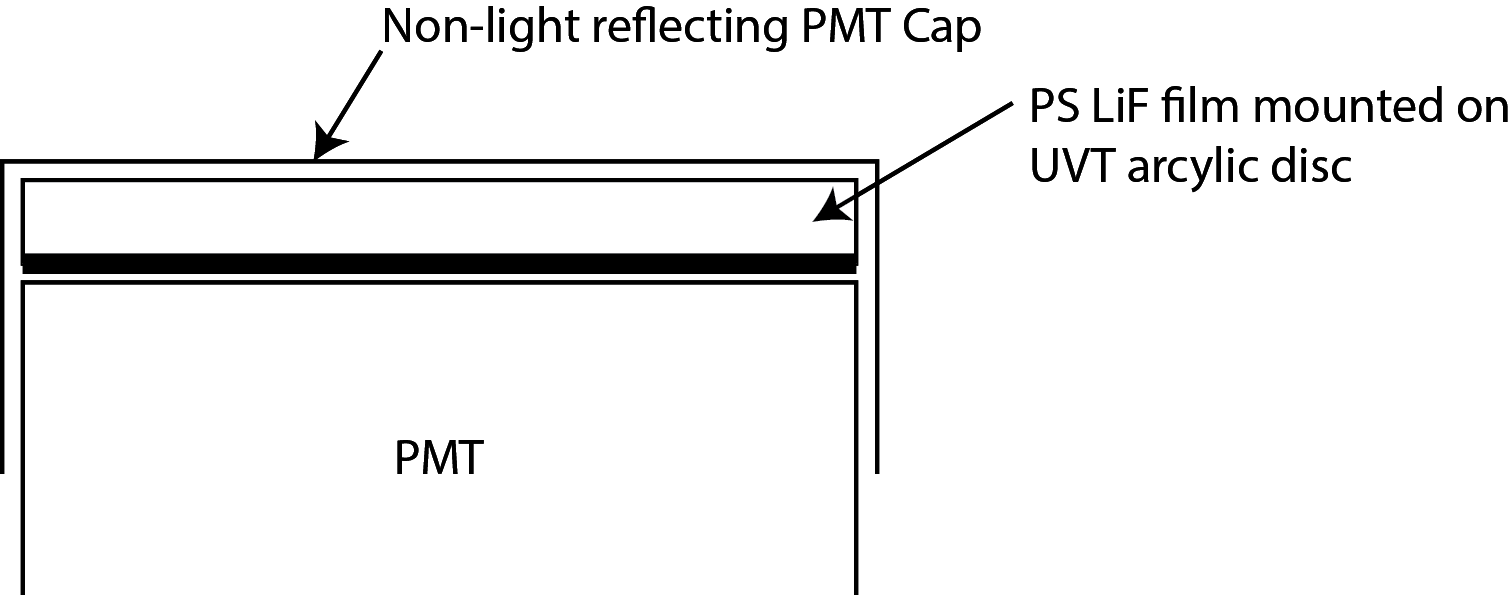
\includegraphics[width=\textwidth]{UVT_PMMA_ExperimentDesign_ExpA}
    \caption{Experiment A}
    \label{fig:ExpA}
  \end{subfigure}%
  ~
  \begin{subfigure}[b]{0.45\textwidth}
    \centering
    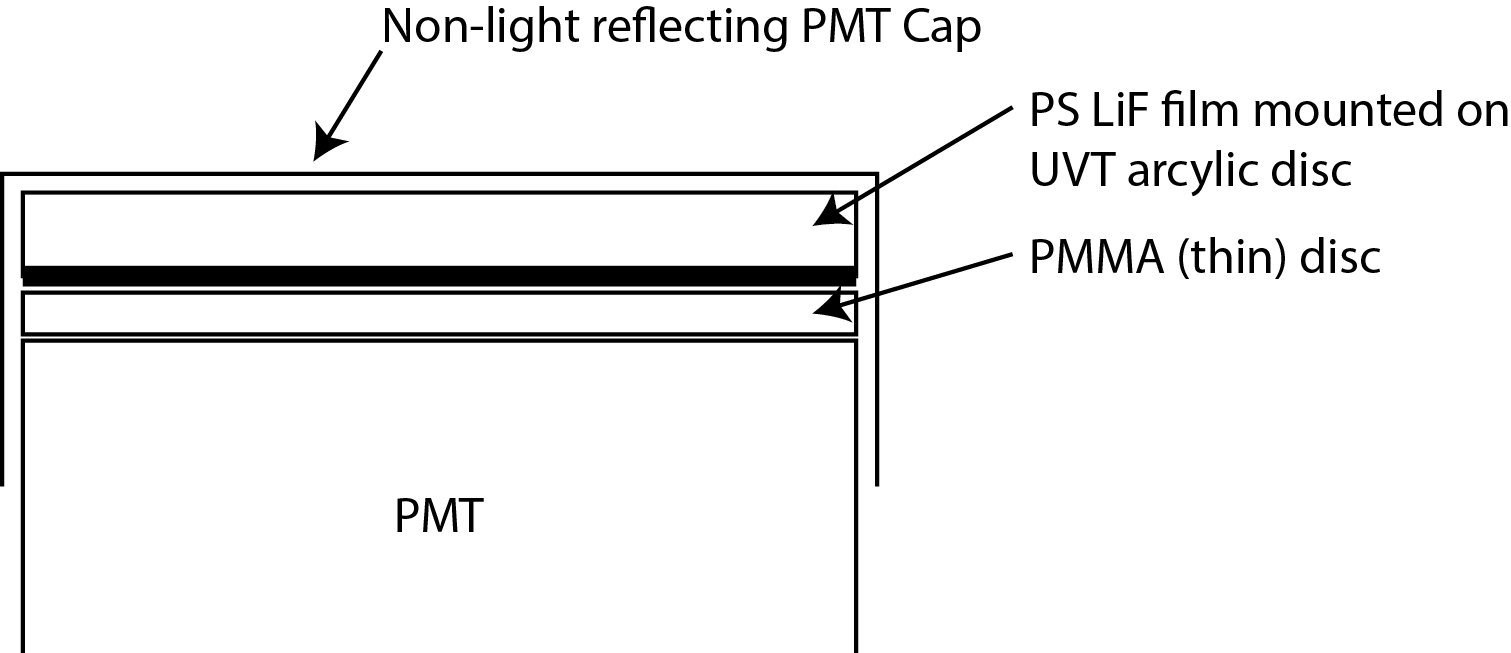
\includegraphics[width=\textwidth]{UVT_PMMA_ExperimentDesign_ExpB}
    \caption{Experiment B}
    \label{fig:ExpB}
  \end{subfigure}%
  
  \begin{subfigure}[b]{0.45\textwidth}
    \centering
    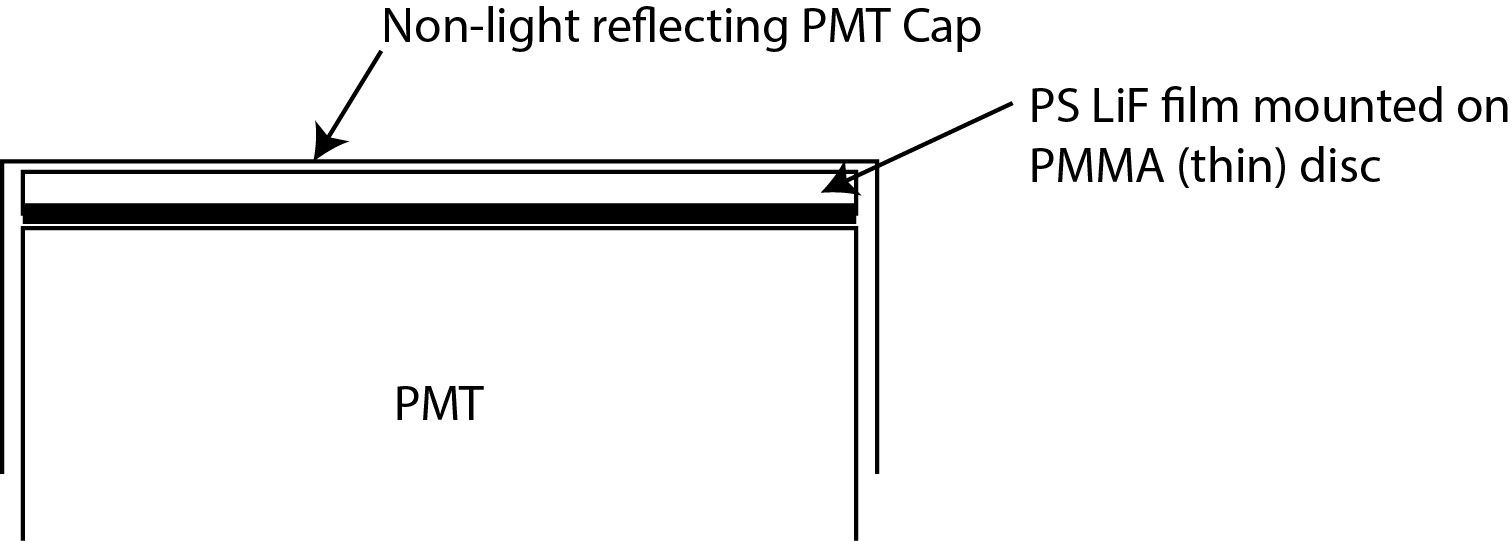
\includegraphics[width=\textwidth]{UVT_PMMA_ExperimentDesign_ExpC}
    \caption{Experiment C}
    \label{fig:ExpC}
  \end{subfigure}%
  ~
  \begin{subfigure}[b]{0.45\textwidth}
    \centering
    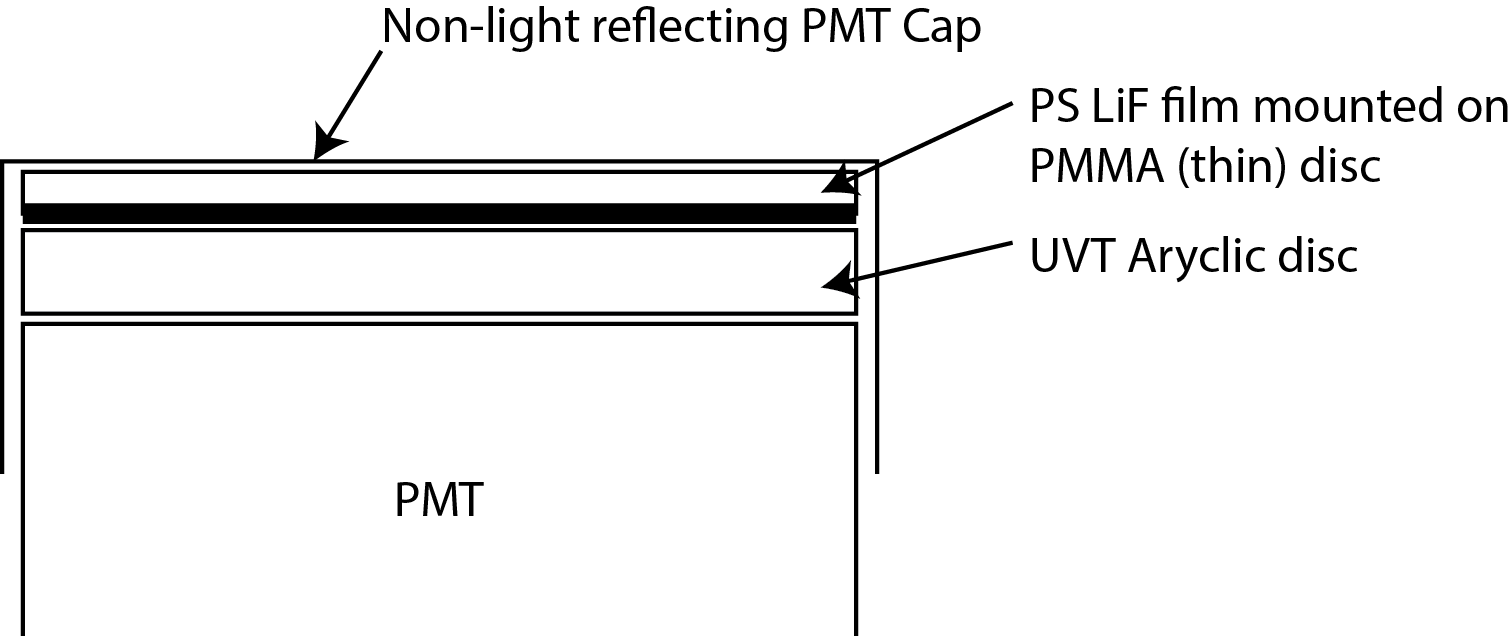
\includegraphics[width=\textwidth]{UVT_PMMA_ExperimentDesign_ExpD}
    \caption{Experiment D}
    \label{fig:ExpD}
  \end{subfigure}
  \caption[Light Attenuation Experiment Design]{Light attenuation experiment design. It was expected that by placing the films in non-reflecting geometry that the light could be forced to be attenuated in a similar manner to being mounted on a PVT Arcylic disc or a PMMA dics.}
  \label{fig:LightAttenExp}
\end{figure}
\subsection{Film Fabrication Experiment}

\section{Results}

It was shown by measurments in a non-reflective geometry by coupling the thin or thick aryclic dics to the film a significant loss in performance (above the loss due to additional layer of optical coupling) is not evident.
\begin{figure}
  \centering
  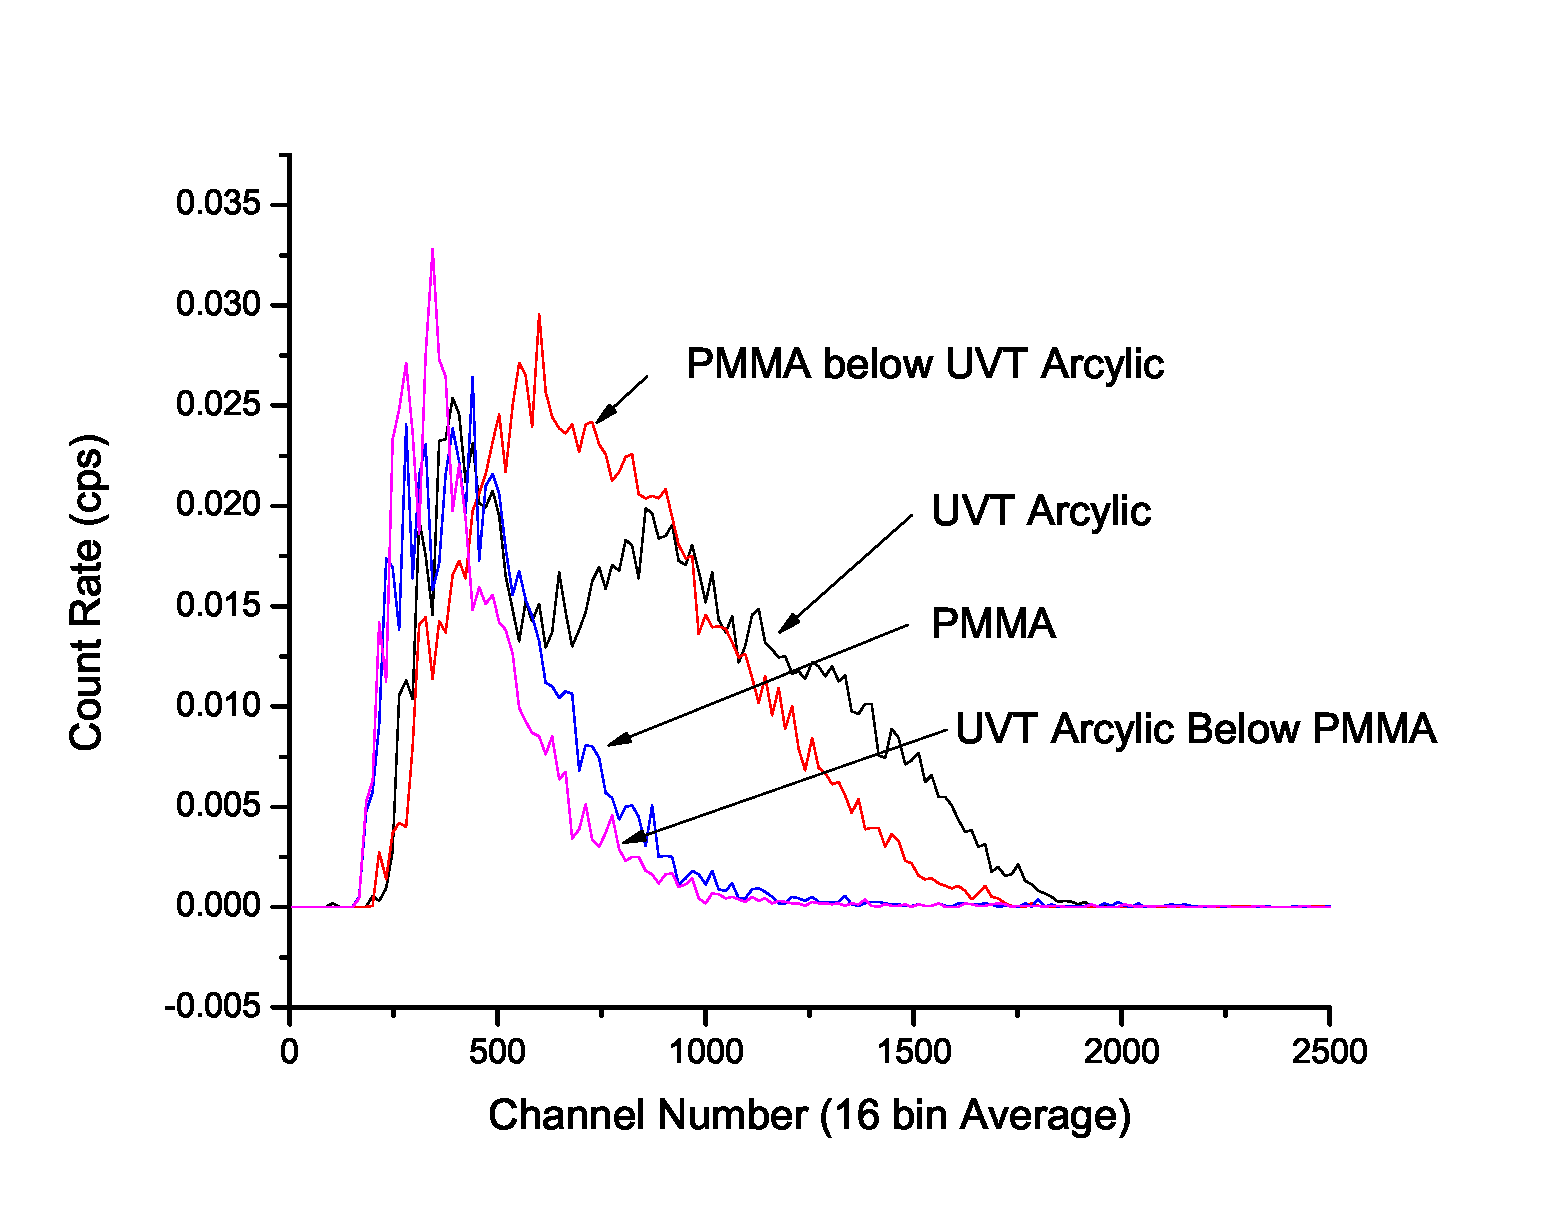
\includegraphics[width=\textwidth]{UVTPMMA_LightYield}
  \caption[Measured Effect of UVT Aryclic and PMMA]{Measured Neutron Spectra of UVT Aryclic and PMMA Films. It is observed that the performance of the thin film is not enhanced by placing it atop of a UVT aryclic disc, and the perfomance of a film cast on a UVT aryclic is not significantly degraded up the placing it on PMMA disc. It is noted that some performance degragation is observed, but it not clear that this is below the effects of adding a additional layer of optical coupling.}
  \label{fig:RadMeasuredExper}
\end{figure}

\section{Conclusions}

It might be best to get away from using the fraction of counts above the discriminator setting, as the denominator is highly dependent on the physical LLD.


\end{document}
